% Options for packages loaded elsewhere
\PassOptionsToPackage{unicode}{hyperref}
\PassOptionsToPackage{hyphens}{url}
%
\documentclass[
]{book}
\usepackage{amsmath,amssymb}
\usepackage{lmodern}
\usepackage{ifxetex,ifluatex}
\ifnum 0\ifxetex 1\fi\ifluatex 1\fi=0 % if pdftex
  \usepackage[T1]{fontenc}
  \usepackage[utf8]{inputenc}
  \usepackage{textcomp} % provide euro and other symbols
\else % if luatex or xetex
  \usepackage{unicode-math}
  \defaultfontfeatures{Scale=MatchLowercase}
  \defaultfontfeatures[\rmfamily]{Ligatures=TeX,Scale=1}
\fi
% Use upquote if available, for straight quotes in verbatim environments
\IfFileExists{upquote.sty}{\usepackage{upquote}}{}
\IfFileExists{microtype.sty}{% use microtype if available
  \usepackage[]{microtype}
  \UseMicrotypeSet[protrusion]{basicmath} % disable protrusion for tt fonts
}{}
\makeatletter
\@ifundefined{KOMAClassName}{% if non-KOMA class
  \IfFileExists{parskip.sty}{%
    \usepackage{parskip}
  }{% else
    \setlength{\parindent}{0pt}
    \setlength{\parskip}{6pt plus 2pt minus 1pt}}
}{% if KOMA class
  \KOMAoptions{parskip=half}}
\makeatother
\usepackage{xcolor}
\IfFileExists{xurl.sty}{\usepackage{xurl}}{} % add URL line breaks if available
\IfFileExists{bookmark.sty}{\usepackage{bookmark}}{\usepackage{hyperref}}
\hypersetup{
  pdftitle={Linear Algebra: An Intuitionist Approach},
  pdfauthor={Matt Pettis},
  hidelinks,
  pdfcreator={LaTeX via pandoc}}
\urlstyle{same} % disable monospaced font for URLs
\usepackage{color}
\usepackage{fancyvrb}
\newcommand{\VerbBar}{|}
\newcommand{\VERB}{\Verb[commandchars=\\\{\}]}
\DefineVerbatimEnvironment{Highlighting}{Verbatim}{commandchars=\\\{\}}
% Add ',fontsize=\small' for more characters per line
\usepackage{framed}
\definecolor{shadecolor}{RGB}{248,248,248}
\newenvironment{Shaded}{\begin{snugshade}}{\end{snugshade}}
\newcommand{\AlertTok}[1]{\textcolor[rgb]{0.94,0.16,0.16}{#1}}
\newcommand{\AnnotationTok}[1]{\textcolor[rgb]{0.56,0.35,0.01}{\textbf{\textit{#1}}}}
\newcommand{\AttributeTok}[1]{\textcolor[rgb]{0.77,0.63,0.00}{#1}}
\newcommand{\BaseNTok}[1]{\textcolor[rgb]{0.00,0.00,0.81}{#1}}
\newcommand{\BuiltInTok}[1]{#1}
\newcommand{\CharTok}[1]{\textcolor[rgb]{0.31,0.60,0.02}{#1}}
\newcommand{\CommentTok}[1]{\textcolor[rgb]{0.56,0.35,0.01}{\textit{#1}}}
\newcommand{\CommentVarTok}[1]{\textcolor[rgb]{0.56,0.35,0.01}{\textbf{\textit{#1}}}}
\newcommand{\ConstantTok}[1]{\textcolor[rgb]{0.00,0.00,0.00}{#1}}
\newcommand{\ControlFlowTok}[1]{\textcolor[rgb]{0.13,0.29,0.53}{\textbf{#1}}}
\newcommand{\DataTypeTok}[1]{\textcolor[rgb]{0.13,0.29,0.53}{#1}}
\newcommand{\DecValTok}[1]{\textcolor[rgb]{0.00,0.00,0.81}{#1}}
\newcommand{\DocumentationTok}[1]{\textcolor[rgb]{0.56,0.35,0.01}{\textbf{\textit{#1}}}}
\newcommand{\ErrorTok}[1]{\textcolor[rgb]{0.64,0.00,0.00}{\textbf{#1}}}
\newcommand{\ExtensionTok}[1]{#1}
\newcommand{\FloatTok}[1]{\textcolor[rgb]{0.00,0.00,0.81}{#1}}
\newcommand{\FunctionTok}[1]{\textcolor[rgb]{0.00,0.00,0.00}{#1}}
\newcommand{\ImportTok}[1]{#1}
\newcommand{\InformationTok}[1]{\textcolor[rgb]{0.56,0.35,0.01}{\textbf{\textit{#1}}}}
\newcommand{\KeywordTok}[1]{\textcolor[rgb]{0.13,0.29,0.53}{\textbf{#1}}}
\newcommand{\NormalTok}[1]{#1}
\newcommand{\OperatorTok}[1]{\textcolor[rgb]{0.81,0.36,0.00}{\textbf{#1}}}
\newcommand{\OtherTok}[1]{\textcolor[rgb]{0.56,0.35,0.01}{#1}}
\newcommand{\PreprocessorTok}[1]{\textcolor[rgb]{0.56,0.35,0.01}{\textit{#1}}}
\newcommand{\RegionMarkerTok}[1]{#1}
\newcommand{\SpecialCharTok}[1]{\textcolor[rgb]{0.00,0.00,0.00}{#1}}
\newcommand{\SpecialStringTok}[1]{\textcolor[rgb]{0.31,0.60,0.02}{#1}}
\newcommand{\StringTok}[1]{\textcolor[rgb]{0.31,0.60,0.02}{#1}}
\newcommand{\VariableTok}[1]{\textcolor[rgb]{0.00,0.00,0.00}{#1}}
\newcommand{\VerbatimStringTok}[1]{\textcolor[rgb]{0.31,0.60,0.02}{#1}}
\newcommand{\WarningTok}[1]{\textcolor[rgb]{0.56,0.35,0.01}{\textbf{\textit{#1}}}}
\usepackage{longtable,booktabs,array}
\usepackage{calc} % for calculating minipage widths
% Correct order of tables after \paragraph or \subparagraph
\usepackage{etoolbox}
\makeatletter
\patchcmd\longtable{\par}{\if@noskipsec\mbox{}\fi\par}{}{}
\makeatother
% Allow footnotes in longtable head/foot
\IfFileExists{footnotehyper.sty}{\usepackage{footnotehyper}}{\usepackage{footnote}}
\makesavenoteenv{longtable}
\usepackage{graphicx}
\makeatletter
\def\maxwidth{\ifdim\Gin@nat@width>\linewidth\linewidth\else\Gin@nat@width\fi}
\def\maxheight{\ifdim\Gin@nat@height>\textheight\textheight\else\Gin@nat@height\fi}
\makeatother
% Scale images if necessary, so that they will not overflow the page
% margins by default, and it is still possible to overwrite the defaults
% using explicit options in \includegraphics[width, height, ...]{}
\setkeys{Gin}{width=\maxwidth,height=\maxheight,keepaspectratio}
% Set default figure placement to htbp
\makeatletter
\def\fps@figure{htbp}
\makeatother
\setlength{\emergencystretch}{3em} % prevent overfull lines
\providecommand{\tightlist}{%
  \setlength{\itemsep}{0pt}\setlength{\parskip}{0pt}}
\setcounter{secnumdepth}{5}
\usepackage{booktabs}
\ifluatex
  \usepackage{selnolig}  % disable illegal ligatures
\fi
\usepackage[]{natbib}
\bibliographystyle{plainnat}

\title{Linear Algebra: An Intuitionist Approach}
\author{Matt Pettis}
\date{2021-10-30}

\usepackage{amsthm}
\newtheorem{theorem}{Theorem}[chapter]
\newtheorem{lemma}{Lemma}[chapter]
\newtheorem{corollary}{Corollary}[chapter]
\newtheorem{proposition}{Proposition}[chapter]
\newtheorem{conjecture}{Conjecture}[chapter]
\theoremstyle{definition}
\newtheorem{definition}{Definition}[chapter]
\theoremstyle{definition}
\newtheorem{example}{Example}[chapter]
\theoremstyle{definition}
\newtheorem{exercise}{Exercise}[chapter]
\theoremstyle{definition}
\newtheorem{hypothesis}{Hypothesis}[chapter]
\theoremstyle{remark}
\newtheorem*{remark}{Remark}
\newtheorem*{solution}{Solution}
\begin{document}
\maketitle

{
\setcounter{tocdepth}{1}
\tableofcontents
}
\hypertarget{preface}{%
\chapter{Preface}\label{preface}}

\begin{quote}
And you may ask yourself, ``What is that beautiful house?''
And you may ask yourself, ``Where does that highway go to?''
And you may ask yourself, ``Am I right? Am I wrong?''
And you may say to yourself, ``My God! What have I done?''

-- Talking Heads, ``Once in a Lifetime''
\end{quote}

\begin{quote}
What one fool can do, another can.

-- Ancient Simian Proverb

-- Sylvanus Thompson, ``Calculus Made Easy''
\end{quote}

\begin{quote}
``Everything is the way it is because it got that way.''

-- D'Arcy Wentworth Thompson
\end{quote}

I'd like to say I'm writing this ``for the democratization of science and math,'' but really, for my kids and their friends so that they don't get snookered into thinking this stuff is beyond them and therefore not for them. It is for you. It is everybody's birthright.

One of the best things about science, but one I've found least talked about in the classes that I took in high school and college, is the part that explains ``why do we think things work this way?'' Why do we believe things are made up of atoms? Why did people believe that without the ability to \emph{see} atoms? What is it about the technology we've built that confirms that things are made of atoms? We believe things like this because we concocted hypotheses and made experimental tests that ruthlessly and cumulatively. We make assumptions that are verifiably true, and then we reach a little further with logic and some more subtle observations, and extend the things we get to conclude, and what we have to throw away. That is a powerful process.

Somewhere along the way, math got divorced from that process. It wasn't helped by great mathematicians like Carl Gauss who called Number Theory ``the Queen of Mathematics'' mostly because it didn't have much in the way of application, and that was a good thing. Or the eminent mathematician G. H. Hardy, who said,

\begin{quote}
``I have never done anything''useful``. No discovery of mine has made, or is likely to make, directly or indirectly, for good or ill, the least difference to the amenity of the world.''
\end{quote}

The perspective was, and often is, that math is a thing more akin to art, like poetry, and though it is sometimes useful, its main value is in that it is beautiful and fun. Ironically, his favorite subject, number theory, is the foundation of our ability to transmit secrets safely on the internet, and does, in fact, probably cause more good and ill than he was comfortable with.

The downside of such a perspective is that it makes it seem like learning the discipline of mathematics is inscrutable. When you encounter mathematical definitions, such as, ``What makes a thing a vector space?'', or ``What makes a thing a group?'', or ``What makes a set measureable?'', what you read are a bunch of seemingly awkward little statements that seem either indecipherable, or unknowable, or so stupidly dead-simple as to make you wonder why one would even need to say such a thing. For instance, when we get to the definition of a vector space, you'll see this as a defining characteristic that your, uh, we'll call a thingy for now, needs to have to be called a vector space:

\[ (\vec{x} + \vec{y}) + \vec{z} = \vec{x} + (\vec{y} + \vec{z}) \]

For those familiar with how numbers work, this seems like something Captain Obvious would say about math. It could also make you wonder ``what's the point of saying such a thing?''

These definitions don't come in an inspiration, like Athena springing fully formed from the forehead of Zeus. When you study the history of mathematics, you'll see that when trying to come up with descriptions like this, mathematicians will often argue, and even disagree violently. You'll often see different characterizations like this depending on where you look, because originators disagreed on what was \emph{fundamental} about what was going on. For systems to be compatible, though, the fundamental assumptions of one camp need to be at least derivable from the other, and vice versa.

This monograph is intended give you the motivations of why linear algebra is the way it is. It will address:

\begin{itemize}
\tightlist
\item
  Where do those rules about a vector space come from?
\item
  What's the big deal about linear independence?
\item
  What would make you come up with an idea like an inner product?
\item
  What's helpful about orthogonality?
\item
  Eigenvectors: how do they even work?
\end{itemize}

I'll approach this as science would ideally approach this. What do we observe? What sort of simplifications can we make to help us understand what is going on? What sort of models help us understand the important parts?

\hypertarget{well-how-did-i-get-here}{%
\chapter{Well, How Did I Get Here?}\label{well-how-did-i-get-here}}

\begin{quote}
Note: I am going to give a physical motivation for vectors here. If you know this pretty well, feel free to skim it.
\end{quote}

Let's dive in by making up a scenario that is half-realistic in the surroundings, and half fantasy in the activities you choose to engage in. The former grounds us in images we can relate to, the latter reminds us that scientists do think of weird things to with their time, and those things are often fruitful to humanity.

Living in Minnesota, you discover that one of the recreations is pushing things around on ice sheets. We are a fascinating lot. So, let's imagine you are on a frozen lake with a liter bottle of vodka. This activity is commonly known as ``ice fishing'' here, though many people never come home with fish.

So you decide to just kick the bottle around for a while before you drink it. While doing this, you make some pretty obvious observations that surprise no one at this point, but for some reason, stick with you. They are:

\begin{itemize}
\tightlist
\item
  The harder you push on the bottle, the faster it ends up going.
\item
  The bottle goes in the direction you push it.
\end{itemize}

Yes, you are a genius for making this observation. As I said, half of the things we do in the story are fantastical things you really wouldn't do with a bottle of vodka on the ice.

Still bored, you decide to try and be more precise about your observations. So, you decide that you will only push on the bottle for one second spans of time. When you do this, you make these observations.

\begin{itemize}
\tightlist
\item
  If you push twice as hard on the bottle, it will end up going twice as fast.
\item
  No matter how hard you push, the bottle still goes in the direction you push it. Generalissimo Francisco Franco is still dead.
\end{itemize}

In this scenario, I assume you have some way of guaging what ``twice as hard'' means. For you physics buffs out there, yes, this is measuring the force you apply to the bottle.

After much hard thinking, you decide to start recording your observations. Since the final speed and direction of the bottle depend only on how hard you push it and what direction you push, you decide to start keeping track of each combination of effort and direction with a drawn arrow.

\begin{figure}

{\centering 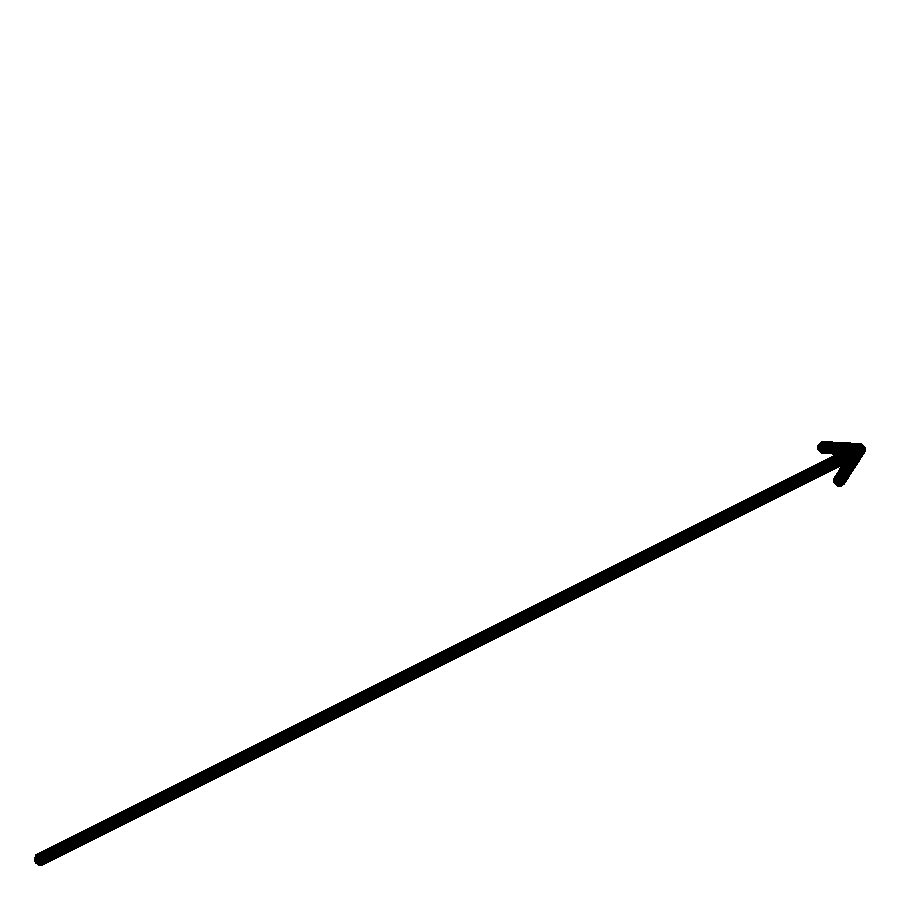
\includegraphics[width=0.5\linewidth,height=0.5\textheight]{images/ch01_single-vector} 

}

\caption{Rockin' Recording System}\label{fig:unnamed-chunk-1}
\end{figure}

An arrow is perfect to capture what you want. You can point it inthe direction you pushed the bottle, and you can make its length correspond to how hard you pushed it. If an arrow is twice as long as another arrow, you pushed it twice as hard.

\textbf{NOTE: RESIST THE TEMPTATION TO LAY A COORDINATE SYSTEM ON THIS YET!} We'll get there, but at this moment, we're not ready to deal with coordinates. We just haven't assembled the tools to figure out how to get there. THIS IS THE RIGHT INTUITION, but we have to do some more work beforehand. It is enough to draw an arrow on a piece of paper in the same direction of the pushed bottle, and draw lengths that record relative magnitudes of how hard you are pushing.

\begin{figure}

{\centering 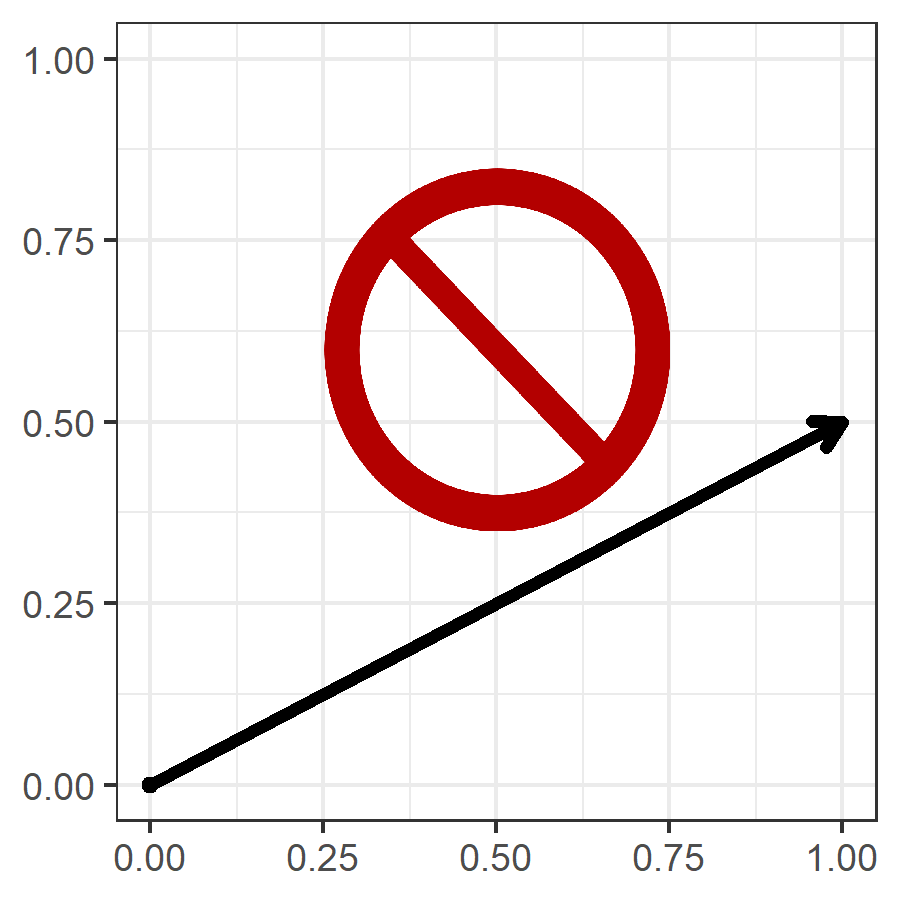
\includegraphics[width=0.5\linewidth,height=0.5\textheight]{images/ch01_single-vector-coords-red-circle-slash} 

}

\caption{DON'T MAKE COORDINATES YET.}\label{fig:unnamed-chunk-2}
\end{figure}

As you do more and more experiments, you notice more things. For instance:

\hypertarget{stopping-what-you-started}{%
\section{Stopping what you started}\label{stopping-what-you-started}}

\begin{itemize}
\tightlist
\item
  The way you stop the bottle dead is to push on it again, in the exact opposite direction.
\end{itemize}

\begin{figure}

{\centering 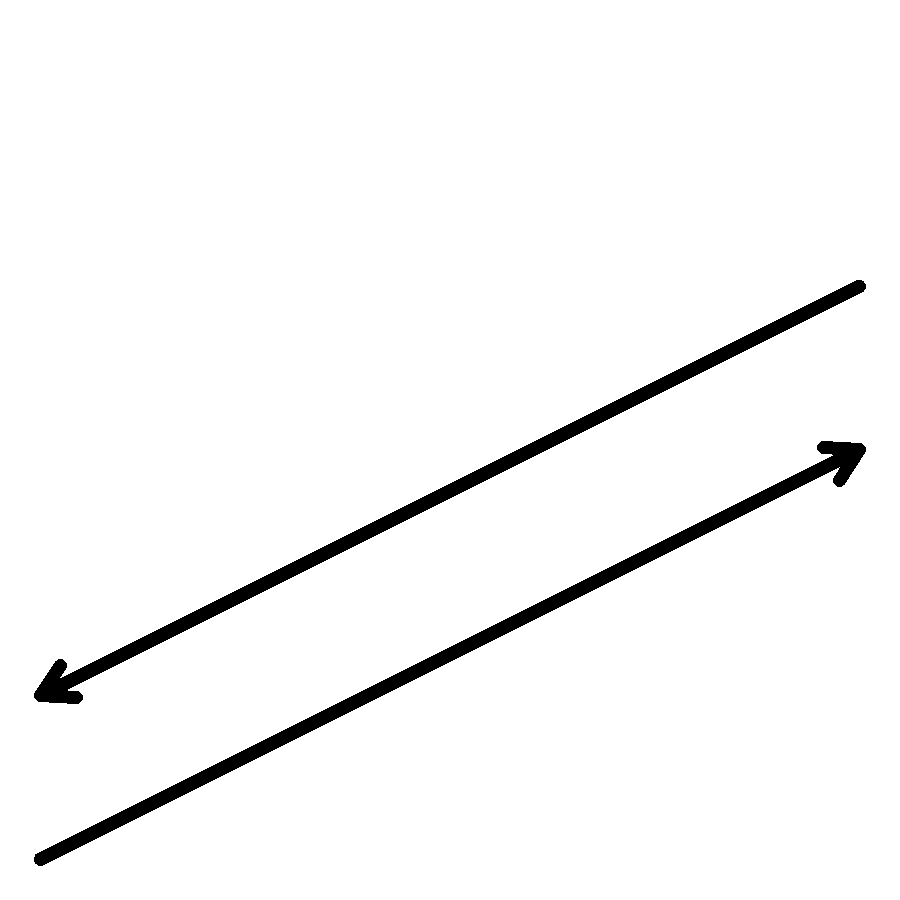
\includegraphics[width=0.5\linewidth,height=0.5\textheight]{images/ch01_additive-inverse} 

}

\caption{Stopping the bottle}\label{fig:unnamed-chunk-3}
\end{figure}

\hypertarget{combo-moves-and-equivalent-move}{%
\section{Combo Moves and Equivalent Move}\label{combo-moves-and-equivalent-move}}

Another thing you notice: you can do combo moves. You can give a push of one size in one direction, then a second sized push in another direction, and that result is the same as if you started with a push of a possibly totally different size in a totally different direction. Well, that's not surprising. What \emph{is} surprising is that if you take your arrow from the first push, and then put the butt of the arrow from the second push at the arrow tip of the first push, and \emph{then} draw an arrow from the start of the first arrow to the end tip of the (moved) second arrow, \emph{that} arrow is the arrow that represents what direction and push size you could have started with to get the same result as you got with the two-combo push you started with.

\begin{figure}

{\centering 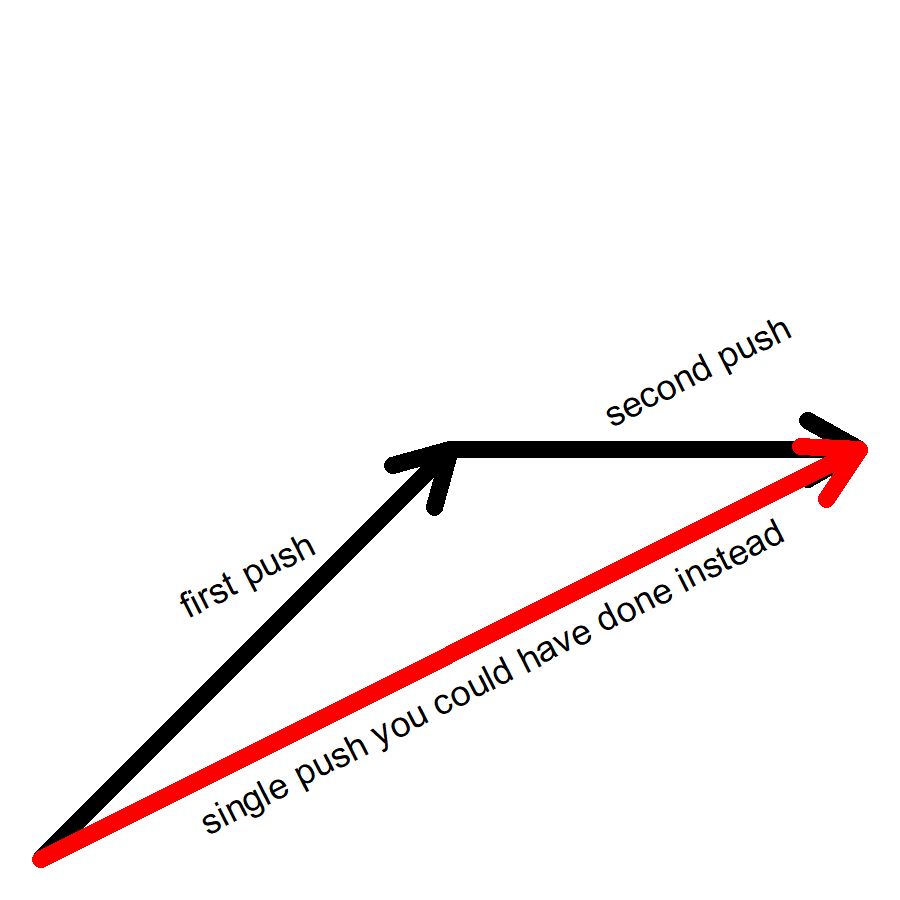
\includegraphics[width=0.5\linewidth,height=0.5\textheight]{images/ch01_three-vector-resultant} 

}

\caption{One push instead of two}\label{fig:unnamed-chunk-4}
\end{figure}

Granted, if you do one push, and afterwards, do a second push, it won't be in the same \emph{line} that a single push would give you, but\ldots{} the two lines would be in the same direction and have the same speed at the end. So we're going to call those equal. That's a big decision, but since no other initial push could give you exactly the same path as the two combo push, it seems to make sense to call those equal.

\hypertarget{order-of-pushing}{%
\section{Order of pushing}\label{order-of-pushing}}

\begin{itemize}
\tightlist
\item
  If you do two pushes in sequence, the result is the same no matter which order you do it in.
\end{itemize}

\begin{figure}

{\centering 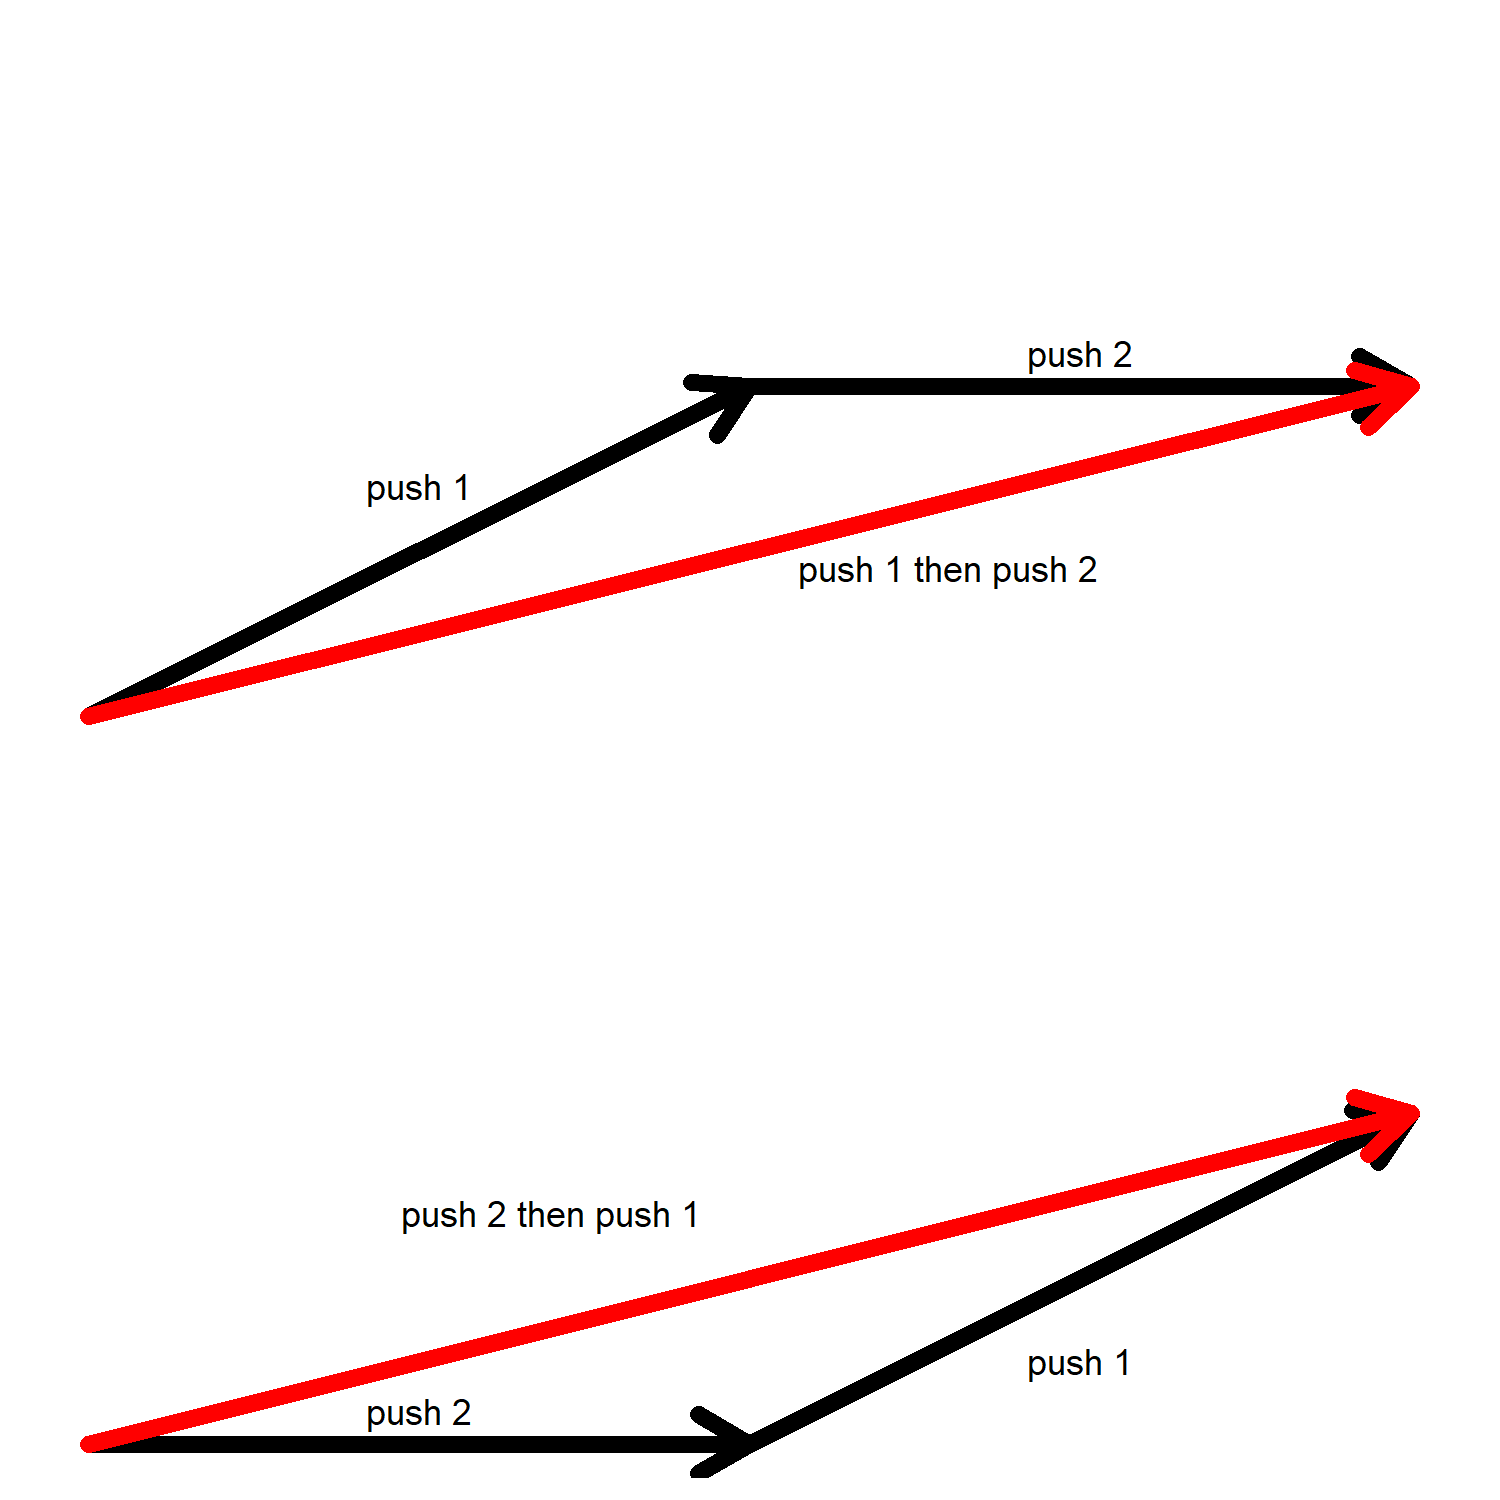
\includegraphics[width=0.5\linewidth,height=0.5\textheight]{images/ch01_push-commutivity} 

}

\caption{Pushing order doesn't matter.}\label{fig:unnamed-chunk-5}
\end{figure}

\hypertarget{the-vector-space-axioms}{%
\section{The Vector Space Axioms}\label{the-vector-space-axioms}}

\begin{figure}

{\centering 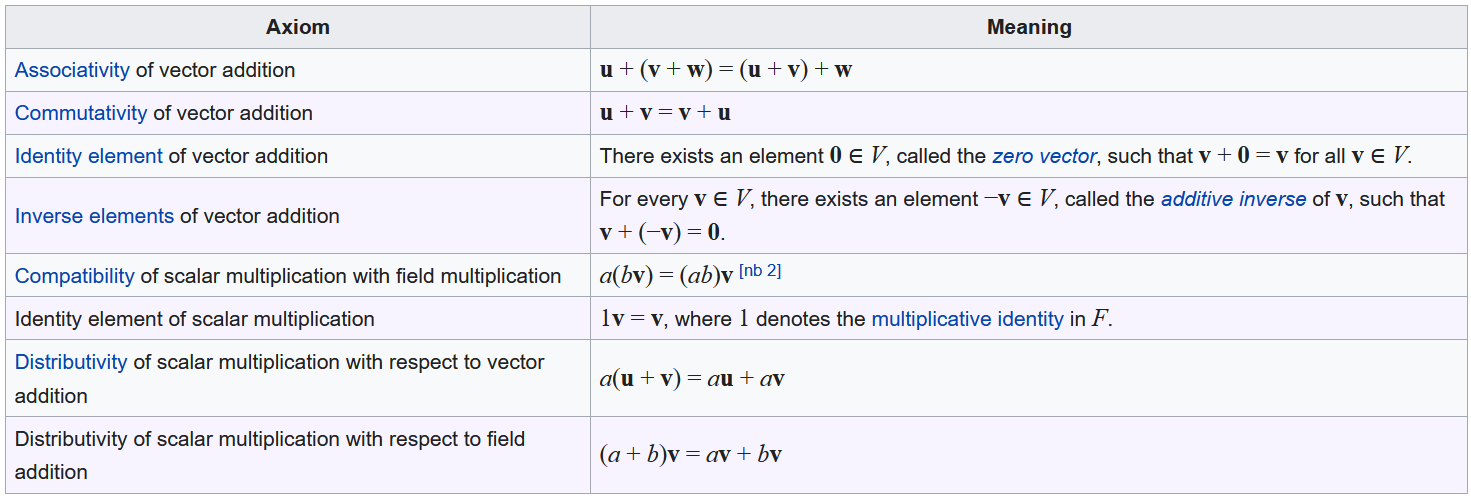
\includegraphics[width=1\linewidth,height=1\textheight]{images/vector-space-axioms-wikipedia} 

}

\caption{Pushing order doesn't matter.}\label{fig:unnamed-chunk-6}
\end{figure}

\hypertarget{cross}{%
\chapter{Cross-references}\label{cross}}

Cross-references make it easier for your readers to find and link to elements in your book.

\hypertarget{chapters-and-sub-chapters}{%
\section{Chapters and sub-chapters}\label{chapters-and-sub-chapters}}

There are two steps to cross-reference any heading:

\begin{enumerate}
\def\labelenumi{\arabic{enumi}.}
\tightlist
\item
  Label the heading: \texttt{\#\ Hello\ world\ \{\#nice-label\}}.

  \begin{itemize}
  \tightlist
  \item
    Leave the label off if you like the automated heading generated based on your heading title: for example, \texttt{\#\ Hello\ world} = \texttt{\#\ Hello\ world\ \{\#hello-world\}}.
  \item
    To label an un-numbered heading, use: \texttt{\#\ Hello\ world\ \{-\#nice-label\}} or \texttt{\{\#\ Hello\ world\ .unnumbered\}}.
  \end{itemize}
\item
  Next, reference the labeled heading anywhere in the text using \texttt{\textbackslash{}@ref(nice-label)}; for example, please see Chapter \ref{cross}.

  \begin{itemize}
  \tightlist
  \item
    If you prefer text as the link instead of a numbered reference use: \protect\hyperlink{cross}{any text you want can go here}.
  \end{itemize}
\end{enumerate}

\hypertarget{captioned-figures-and-tables}{%
\section{Captioned figures and tables}\label{captioned-figures-and-tables}}

Figures and tables \emph{with captions} can also be cross-referenced from elsewhere in your book using \texttt{\textbackslash{}@ref(fig:chunk-label)} and \texttt{\textbackslash{}@ref(tab:chunk-label)}, respectively.

See Figure \ref{fig:nice-fig}.

\begin{Shaded}
\begin{Highlighting}[]
\FunctionTok{par}\NormalTok{(}\AttributeTok{mar =} \FunctionTok{c}\NormalTok{(}\DecValTok{4}\NormalTok{, }\DecValTok{4}\NormalTok{, .}\DecValTok{1}\NormalTok{, .}\DecValTok{1}\NormalTok{))}
\FunctionTok{plot}\NormalTok{(pressure, }\AttributeTok{type =} \StringTok{\textquotesingle{}b\textquotesingle{}}\NormalTok{, }\AttributeTok{pch =} \DecValTok{19}\NormalTok{)}
\end{Highlighting}
\end{Shaded}

\begin{figure}

{\centering 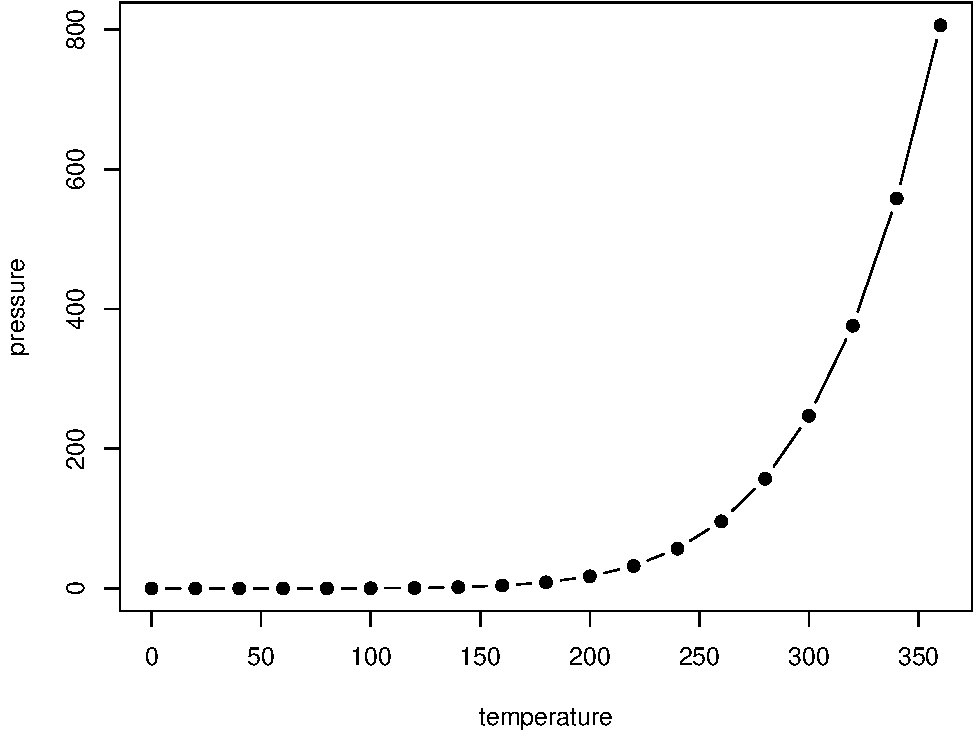
\includegraphics[width=0.8\linewidth]{_main_files/figure-latex/nice-fig-1} 

}

\caption{Here is a nice figure!}\label{fig:nice-fig}
\end{figure}

Don't miss Table \ref{tab:nice-tab}.

\begin{Shaded}
\begin{Highlighting}[]
\NormalTok{knitr}\SpecialCharTok{::}\FunctionTok{kable}\NormalTok{(}
  \FunctionTok{head}\NormalTok{(pressure, }\DecValTok{10}\NormalTok{), }\AttributeTok{caption =} \StringTok{\textquotesingle{}Here is a nice table!\textquotesingle{}}\NormalTok{,}
  \AttributeTok{booktabs =} \ConstantTok{TRUE}
\NormalTok{)}
\end{Highlighting}
\end{Shaded}

\begin{table}

\caption{\label{tab:nice-tab}Here is a nice table!}
\centering
\begin{tabular}[t]{rr}
\toprule
temperature & pressure\\
\midrule
0 & 0.0002\\
20 & 0.0012\\
40 & 0.0060\\
60 & 0.0300\\
80 & 0.0900\\
\addlinespace
100 & 0.2700\\
120 & 0.7500\\
140 & 1.8500\\
160 & 4.2000\\
180 & 8.8000\\
\bottomrule
\end{tabular}
\end{table}

\hypertarget{parts}{%
\chapter{Parts}\label{parts}}

You can add parts to organize one or more book chapters together. Parts can be inserted at the top of an .Rmd file, before the first-level chapter heading in that same file.

Add a numbered part: \texttt{\#\ (PART)\ Act\ one\ \{-\}} (followed by \texttt{\#\ A\ chapter})

Add an unnumbered part: \texttt{\#\ (PART\textbackslash{}*)\ Act\ one\ \{-\}} (followed by \texttt{\#\ A\ chapter})

Add an appendix as a special kind of un-numbered part: \texttt{\#\ (APPENDIX)\ Other\ stuff\ \{-\}} (followed by \texttt{\#\ A\ chapter}). Chapters in an appendix are prepended with letters instead of numbers.

\hypertarget{footnotes-and-citations}{%
\chapter{Footnotes and citations}\label{footnotes-and-citations}}

\hypertarget{footnotes}{%
\section{Footnotes}\label{footnotes}}

Footnotes are put inside the square brackets after a caret \texttt{\^{}{[}{]}}. Like this one \footnote{This is a footnote.}.

\hypertarget{citations}{%
\section{Citations}\label{citations}}

Reference items in your bibliography file(s) using \texttt{@key}.

For example, we are using the \textbf{bookdown} package \citep{R-bookdown} (check out the last code chunk in index.Rmd to see how this citation key was added) in this sample book, which was built on top of R Markdown and \textbf{knitr} \citep{xie2015} (this citation was added manually in an external file book.bib).
Note that the \texttt{.bib} files need to be listed in the index.Rmd with the YAML \texttt{bibliography} key.

The RStudio Visual Markdown Editor can also make it easier to insert citations: \url{https://rstudio.github.io/visual-markdown-editing/\#/citations}

\hypertarget{blocks}{%
\chapter{Blocks}\label{blocks}}

\hypertarget{equations}{%
\section{Equations}\label{equations}}

Here is an equation.

\begin{equation} 
  f\left(k\right) = \binom{n}{k} p^k\left(1-p\right)^{n-k}
  \label{eq:binom}
\end{equation}

You may refer to using \texttt{\textbackslash{}@ref(eq:binom)}, like see Equation \eqref{eq:binom}.

\hypertarget{theorems-and-proofs}{%
\section{Theorems and proofs}\label{theorems-and-proofs}}

Labeled theorems can be referenced in text using \texttt{\textbackslash{}@ref(thm:tri)}, for example, check out this smart theorem \ref{thm:tri}.

\begin{theorem}
\protect\hypertarget{thm:tri}{}\label{thm:tri}For a right triangle, if \(c\) denotes the \emph{length} of the hypotenuse
and \(a\) and \(b\) denote the lengths of the \textbf{other} two sides, we have
\[a^2 + b^2 = c^2\]
\end{theorem}

Read more here \url{https://bookdown.org/yihui/bookdown/markdown-extensions-by-bookdown.html}.

\hypertarget{callout-blocks}{%
\section{Callout blocks}\label{callout-blocks}}

The R Markdown Cookbook provides more help on how to use custom blocks to design your own callouts: \url{https://bookdown.org/yihui/rmarkdown-cookbook/custom-blocks.html}

\hypertarget{sharing-your-book}{%
\chapter{Sharing your book}\label{sharing-your-book}}

\hypertarget{publishing}{%
\section{Publishing}\label{publishing}}

HTML books can be published online, see: \url{https://bookdown.org/yihui/bookdown/publishing.html}

\hypertarget{pages}{%
\section{404 pages}\label{pages}}

By default, users will be directed to a 404 page if they try to access a webpage that cannot be found. If you'd like to customize your 404 page instead of using the default, you may add either a \texttt{\_404.Rmd} or \texttt{\_404.md} file to your project root and use code and/or Markdown syntax.

\hypertarget{metadata-for-sharing}{%
\section{Metadata for sharing}\label{metadata-for-sharing}}

Bookdown HTML books will provide HTML metadata for social sharing on platforms like Twitter, Facebook, and LinkedIn, using information you provide in the \texttt{index.Rmd} YAML. To setup, set the \texttt{url} for your book and the path to your \texttt{cover-image} file. Your book's \texttt{title} and \texttt{description} are also used.

This \texttt{gitbook} uses the same social sharing data across all chapters in your book- all links shared will look the same.

Specify your book's source repository on GitHub using the \texttt{edit} key under the configuration options in the \texttt{\_output.yml} file, which allows users to suggest an edit by linking to a chapter's source file.

Read more about the features of this output format here:

\url{https://pkgs.rstudio.com/bookdown/reference/gitbook.html}

Or use:

\begin{Shaded}
\begin{Highlighting}[]
\NormalTok{?bookdown}\SpecialCharTok{::}\NormalTok{gitbook}
\end{Highlighting}
\end{Shaded}


  \bibliography{book.bib,packages.bib}

\end{document}
